%% LyX 2.2.4 created this file.  For more info, see http://www.lyx.org/.
%% Do not edit unless you really know what you are doing.
\documentclass[english]{article}
\usepackage{lmodern}
\usepackage[T1]{fontenc}
\usepackage[latin9]{inputenc}
\usepackage{geometry}
\geometry{verbose,tmargin=3cm,bmargin=3cm,lmargin=2.5cm,rmargin=2.5cm}
\usepackage{textcomp}
\usepackage{amstext}
\usepackage{graphicx}
\usepackage{pdfpages}


\makeatletter

%%%%%%%%%%%%%%%%%%%%%%%%%%%%%% LyX specific LaTeX commands.
%% Because html converters don't know tabularnewline
\providecommand{\tabularnewline}{\\}

\makeatother

\usepackage{babel}
\begin{document}


\includepdf[pages=-]{SSD.pdf}
\setcounter{page}{1}

\title{3F8: Inference\\
 Short Lab Report}

\author{Jack Henry\\
crsid: jbh48}
\maketitle


\begin{abstract}
This report investigates the use of logistic regression for binary classification and explores the limitations of linear models on non-linearly separable data. The model is optimized using gradient ascent, and Gaussian radial basis functions are introduced to capture non-linear decision boundaries. The results show that while the logistic regression model performs reasonably well, the introduction of radial basis functions improves generalization and reduces overfitting, though further improvements are still needed for better classification accuracy.
\end{abstract}

\section{Introduction}
\begin{enumerate}
\item Binary classification using logistic regression is a fundamental technique in statistical inference and machine learning. Logistic regression is widely used due to its interpretability and efficiency, modeling probabilities directly, allowing for probabilistic decision-making rather than just hard classifications. Understanding how to optimize its parameters and evaluate its performance is crucial for developing reliable predictive models.
\item This report follows up by implementing logistic regression using gradient ascent, evaluating its performance on a given dataset, and extending the model with Gaussian radial basis functions to explore non-linear decision boundaries. The effectiveness of these approaches is assessed through log-likelihood analysis, confusion matrices, and decision boundary visualizations.
\end{enumerate}

\section{Exercise a)\label{sec:Exercise-a}}

In this exercise we have to consider the logistic classification model
(aka logistic regression) and derive the gradients of the log-likelihood
given a vector of binary labels $\mathbf{y}$ and a matrix of input
features $\mathbf{X}$. The gradient of the log-likelihood can be
written as
\begin{equation}
\frac{\partial\mathcal{L}(\boldsymbol{\beta})}{\partial\boldsymbol{\beta}} = \mathbf{X}^T (\mathbf{y} - \sigma(\mathbf{X} \boldsymbol{\beta}))
\end{equation}


\section{Exercise b)}

In this exercise we are asked to write pseudocode to estimate the
parameters $\beta$ using gradient ascent of the log-likelihood. Our
code should be vectorised. The pseudocode to estimate the parameters
$\beta$ is shown below:
\newpage
\begin{verbatim}
Function estimate_parameters:

   Input:  feature matrix X, labels y
   Output: vector of coefficients b
	
   Code:

      Initialize b randomly
      Set learning_rate
      Set n_steps

      For i = 1 to n_steps do:
         p = sigmoid(X * b)
         gradient = X' * (y - p)
         b = b + learning_rate * gradient

      return b
\end{verbatim}

The learning rate parameter $\eta$ is chosen through trial and error. The final value is chosen for a mixture of clarity for visual representation, and accuracy of the model. The average log-likelihood curves need to plateau to ideally a steady value for an accurate model, and a visible curve at the start is useful to show the iterative process used. An iterative technique was also used to find the fastest converging learning rate, however this was not useful to visually show the concepts and ideas of the methods used.

\section{Exercise c)}

In this exercise we visualise the dataset in the two-dimensional input
space displaying each datapoint's class label. The dataset is visualised
in Figure \ref{fig:data_visualisation}. By analyzing Figure \ref{fig:data_visualisation}, we conclude that a linear classifier is unlikely to perform well, as the decision boundary appears to be non-linear. The data points form a structure that suggests a more complex decision function is needed to separate the classes effectively.

\begin{figure} [htbp]
\begin{centering}
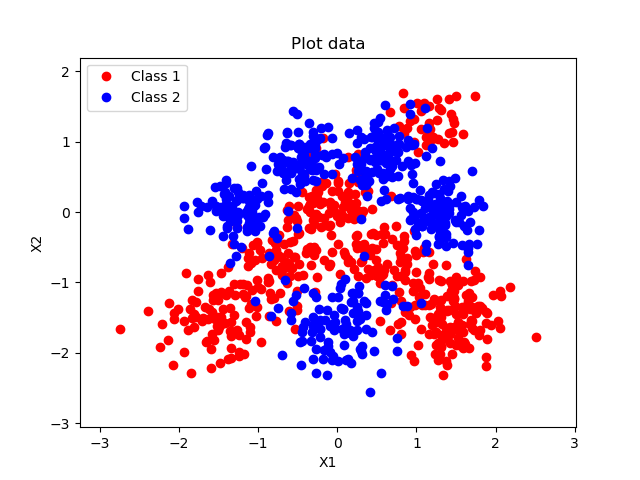
\includegraphics[width=0.3\paperwidth]{Data_Visualisation.png}
\par\end{centering}
\caption{Visualisation of the data.\label{fig:data_visualisation} }
\end{figure}


\section{Exercise d)}

In this exercise we split the data randomly into training and test
sets with 800 and 200 data points, respectively. The pseudocode from
exercise a) is transformed into python code as follows:
\begin{verbatim}

def logistic(x): 
    return 1.0 / (1.0 + np.exp(-x))

def predict(X_tilde, w): 
    return logistic(np.dot(X_tilde, w))
    
def fit_w(X_tilde_train, y_train, X_tilde_test, y_test, n_steps, alpha):
    w = np.random.randn(X_tilde_train.shape[ 1 ]) 
    ll_train = np.zeros(n_steps) 
    ll_test = np.zeros(n_steps) 
    for i in range(n_steps):
        sigmoid_value = predict(X_tilde_train, w)
        gradient = X_tilde_train.T @ (y_train - sigmoid_value)
        w = w + alpha * gradient  # Gradient-based update rule for w
        ll_train[ i ] = compute_average_ll(X_tilde_train, y_train, w) 
        ll_test[ i ] = compute_average_ll(X_tilde_test, y_test, w) 
    return w, ll_train, ll_test 
\end{verbatim}
We then train the classifier using this code. We fixed the learning
rate parameter to be $\eta=0.00005$. The average log-likelihood on the
training and test sets as the optimisation proceeds are shown in Figure
\ref{fig:learning_curves}. By looking at these plots, we conclude that the model has successfully learned from the data in a reasonable number of steps without overfitting, as the training and test log-likelihoods settle to similar values. However, the final log-likelihood is relatively low, suggesting that a linear classifier may not be the best fit for this dataset, given its non-linear structure. 

Figure \ref{fig:data_visualisation-1} displays the visualisation of the contours of the class predictive probabilities on top of the data. This figure shows that the model has learned a linear decision boundary, resulting in smooth probability transitions between classes. However, due to the non-linear nature of the dataset, the classifier struggles to separate the two classes effectively, leading to misclassified points.

\begin{figure} [htbp]
\begin{centering}
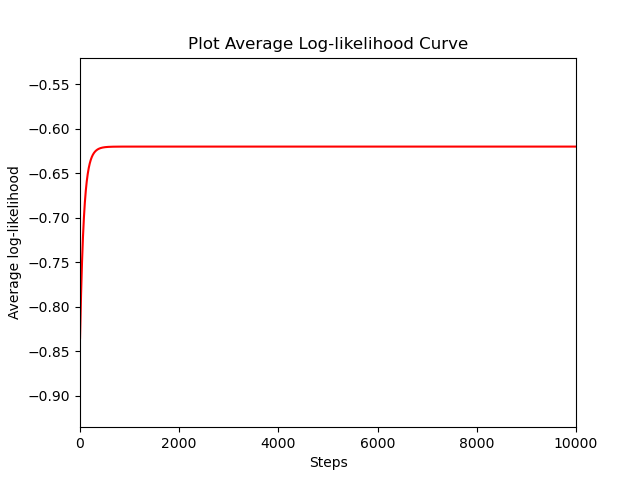
\includegraphics[width=0.3\paperwidth]{Training_LL.png}\hspace{1cm}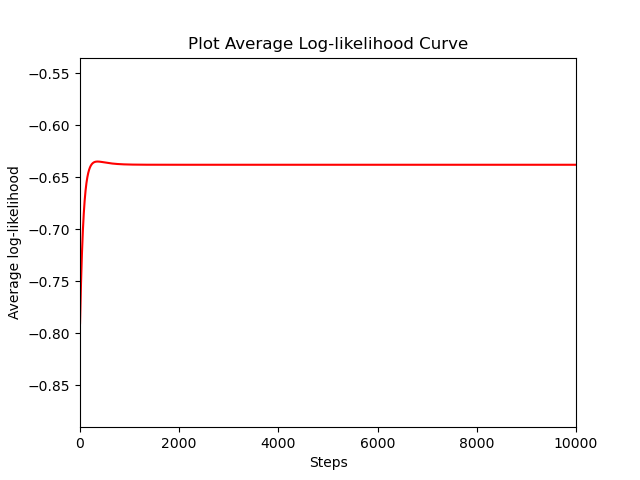
\includegraphics[width=0.3\paperwidth]{Test_LL.png}
\par\end{centering}
\caption{Learning curves showing the average log-likelihood on the training
(left) and test (right) datasets.\label{fig:learning_curves} }
\end{figure}

\begin{figure} [htbp]
\begin{centering}
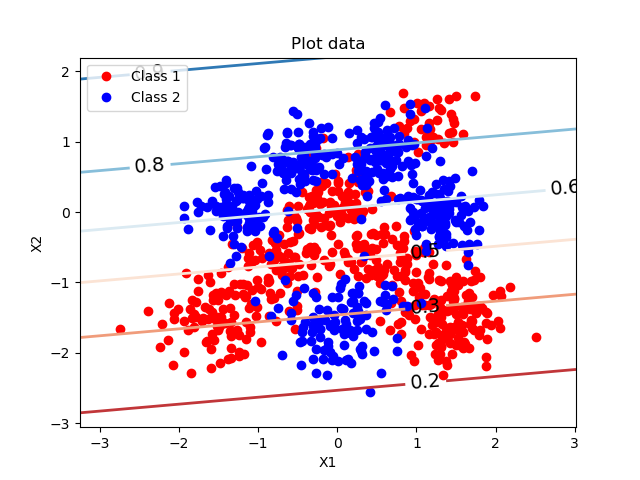
\includegraphics[width=0.3\paperwidth]{Linear_classifier_contour.png}
\par\end{centering}
\caption{Visualisation of the contours of the class predictive probabilities.\label{fig:data_visualisation-1} }
\end{figure}


\section{Exercise e)}

The final average training and test log-likelihoods are shown in Table
\ref{tab:average_ll}. These results indicate that there is little to no overfitting, as both training and testing values are similar, however, the final log-likelihood values are relatively low, suggesting that a linear classifier may not be the best fit for this dataset.
The 2x2 confusion
matrices on the and test set is shown in Table \ref{tab:confusion_test}.
By analyzing this table, we conclude that the logistic regression model performs reasonably well in terms of predicting the majority of the class labels, however, the model still shows a reasonable amount of misclassifications. These errors suggest that the linear decision boundary used by the logistic regression model is not ideal for this dataset. Given the apparent non-linear structure of the data, a more complex model or feature expansion may be necessary to improve classification accuracy and capture the true decision boundary more effectively.

\begin{table} [htbp]
\centering{}%
\begin{minipage}[t]{0.49\columnwidth}%
\begin{center}
\begin{tabular}{c|c}
\textbf{Avg. Train ll} & \textbf{Avg. Test ll}\tabularnewline
\hline 
-0.6202 & -0.6380\tabularnewline
\hline 
\end{tabular} 
\par\end{center}
\caption{Average training and test log-likelihoods.\label{tab:average_ll}}
%
\end{minipage}%
\begin{minipage}[t]{0.49\columnwidth}%
\begin{center}
\begin{tabular}{cc|c|c}
 & \multicolumn{1}{c}{} & \multicolumn{1}{c}{$\hat{y}$} & \tabularnewline
 &  & 0 & 1\tabularnewline
\cline{2-4} 
$y$ & 0 & 0.6972 & 0.3028\tabularnewline
\cline{2-4} 
 & 1 & 0.2637 & 0.7363\tabularnewline
\cline{2-4} 
\end{tabular} 
\par\end{center}
\caption{Confusion matrix on the test set.\label{tab:confusion_test}}
%
\end{minipage}
\end{table}


\section{Exercise f)}

We now expand the inputs through a set of Gaussian radial basis functions
centred on the training datapoints. We consider widths $l=\{0.01,0.1,1\}$
for the basis functions. We fix the learning rate parameter to be
$\eta=\{0.005, 0.0008, 0.00005\}$ for each $l=\{0.01,0.1,1\}$, respectively.
Figure \ref{fig:contours_l} displays the visualisation of the contours
of the resulting class predictive probabilities on top of the data
for each choice of $l=\{0.01,0.1,1\}$.
\begin{figure} [htpb]
\begin{centering}
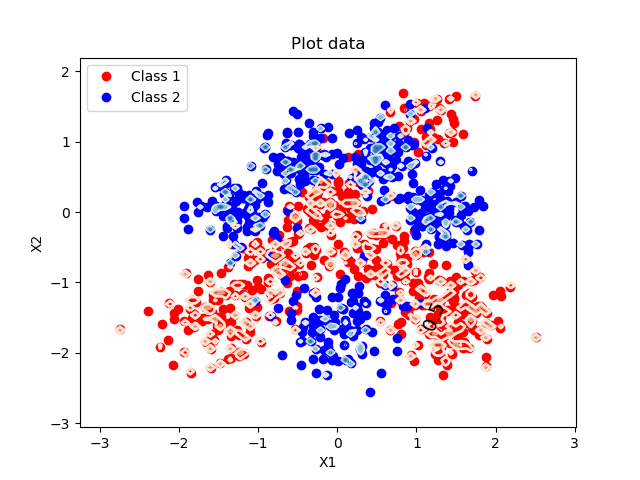
\includegraphics[width=0.32\textwidth]{RBF_0.01.png}\hspace{0.15cm}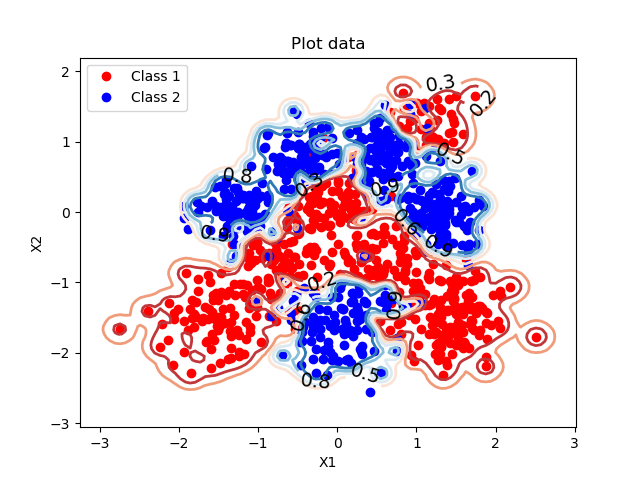
\includegraphics[width=0.32\textwidth]{RBF_0.1.png}\hspace{0.15cm}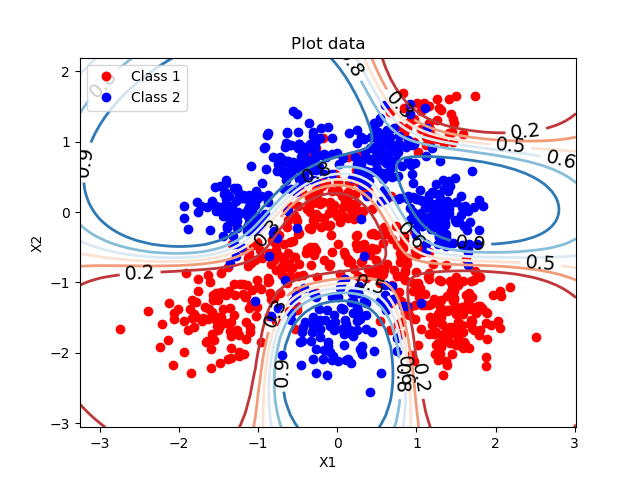
\includegraphics[width=0.32\textwidth]{RBF_1.png}
\par\end{centering}
\caption{Visualisation of the contours of the class predictive probabilities
for $l=0.01$ (left), $l=0.1$ (middle), $l=1$ (right).\label{fig:contours_l} }
\end{figure}


\section{Exercise g)}

The final training and test log-likelihoods per datapoint obtained
for each setting of $l=\{0.01,0.1,1\}$ are shown in tables \ref{tab:avg_ll_l_001},
\ref{tab:avg_ll_l_01} and \ref{tab:avg_ll_l_1}. 

These results indicate that as the width parameter $l$ increases, the average test log-likelihood improves. With $l = 0.01$ the model seems to harshly overfit, as seen in the high discrepancy between training and test log-likelihoods. This could also be seen in the log-likelihood curves, with the average log-likelihood decreasing with the number of steps. As $l$ increases from 0.01 to 0.1 and 1, i.e. the basis functions get 'wider', the model generalizes better with smaller gaps between training and test log-likelihoods, indicating improved performance on the test set. The model trained with $l = 1$ actually performs better on the test set than it does on the training set, suggesting that the model is effectively regularized. 

The 2 \texttimes{} 2 confusion matrices for the three models trained with $l=\{0.01,0.1,1\}$ are show in tables \ref{tab:conf_l_001},
\ref{tab:conf_l_01} and \ref{tab:conf_l_1}. After analyzing these matrices, we can say that as $l$ increases, the classifier becomes more conservative in predicting the positive class (1). With $l = 0.01$, the model is overly confident in predicting class 0, even when class 1 is the true label, leading to a higher rate of both true and false negatives. As $l$ increases, the model becomes more balanced, with fewer misclassifications of class 1, but the tendency to misclassify class 0 as class 1 increases, especially for $l = 1$. This shift reflects the impact of regularization on reducing overfitting and encouraging more conservative predictions.

When we compare these results to those obtained using the original inputs, we conclude that increasing the width of the RBFs helps to mitigate overfitting and improves generalization. The results with $l = 0.01$ show a tendency to overfit, which is reduced as $l$ increases. The classifier with wider RBFs ($l = 1$) achieves a better balance between training and test performance, and the confusion matrices indicate improved classification of the positive class. Increasing $l$ seems to make the model more robust, although there is still room for improvement, particularly in minimizing misclassifications of class 0.

\begin{table} [htbp]
\centering{}%
\begin{minipage}[t]{0.3\textwidth}%
\begin{center}
\begin{tabular}{c|c}
\textbf{Avg. Train ll} & \textbf{Avg. Test ll}\tabularnewline
\hline 
-0.0208 & -0.6762\tabularnewline
\hline 
\end{tabular}\caption{Results for $l=0.01$\label{tab:avg_ll_l_001}}
\par\end{center}%
\end{minipage}\hspace{0.5cm}%
\begin{minipage}[t]{0.3\textwidth}%
\begin{center}
\begin{tabular}{c|c}
\textbf{Avg. Train ll} & \textbf{Avg. Test ll}\tabularnewline
\hline 
-0.0997 & -0.2627\tabularnewline
\hline 
\end{tabular}\caption{Results for $l=0.1$\label{tab:avg_ll_l_01}}
\par\end{center}%
\end{minipage}\hspace{0.5cm}%
\begin{minipage}[t]{0.3\textwidth}%
\begin{center}
\begin{tabular}{c|c}
\textbf{Avg. Train ll} & \textbf{Avg. Test ll}\tabularnewline
\hline 
-0.2169 & -0.2054\tabularnewline
\hline 
\end{tabular}\caption{Results for $l=1$\label{tab:avg_ll_l_1}}
\par\end{center}%
\end{minipage}
\end{table}

\begin{table} [htbp]
\centering{}%
\begin{minipage}[t]{0.33\textwidth}%
\begin{center}
\begin{tabular}{cc|c|c}
 & \multicolumn{1}{c}{} & \multicolumn{1}{c}{$\hat{y}$} & \tabularnewline
 &  & 0 & 1\tabularnewline
\cline{2-4} 
$y$ & 0 & 0.9817 & 0.0183\tabularnewline
\cline{2-4} 
 & 1 & 0.8791 & 0.1209\tabularnewline
\cline{2-4} 
\end{tabular} 
\par\end{center}
\caption{Conf. matrix $l=0.01$.\label{tab:conf_l_001}}
%
\end{minipage}%
\begin{minipage}[t]{0.33\textwidth}%
\begin{center}
\begin{tabular}{cc|c|c}
 & \multicolumn{1}{c}{} & \multicolumn{1}{c}{$\hat{y}$} & \tabularnewline
 &  & 0 & 1\tabularnewline
\cline{2-4} 
$y$ & 0 & 0.9174 & 0.0826\tabularnewline
\cline{2-4} 
 & 1 & 0.1429 & 0.8571\tabularnewline
\cline{2-4} 
\end{tabular} 
\par\end{center}
\caption{Conf. matrix $l=0.1$.\label{tab:conf_l_01}}
%
\end{minipage}%
\begin{minipage}[t]{0.33\textwidth}%
\begin{center}
\begin{tabular}{cc|c|c}
 & \multicolumn{1}{c}{} & \multicolumn{1}{c}{$\hat{y}$} & \tabularnewline
 &  & 0 & 1\tabularnewline
\cline{2-4} 
$y$ & 0 & 0.8899 & 0.1101\tabularnewline
\cline{2-4} 
 & 1 & 0.0549 & 0.9451\tabularnewline
\cline{2-4} 
\end{tabular} 
\par\end{center}
\caption{Conf. matrix $l=1$.\label{tab:conf_l_1}}
%
\end{minipage}
\end{table}


\section{Conclusions} 
\begin{enumerate}
    \item \textbf{Summary of Results and Consequences} \\
    In this study, we implemented a logistic regression classifier and evaluated its performance on a given binary classification dataset. The key findings include:
    \begin{itemize}
         \item The performance of the linear logistic regression model was suboptimal for this dataset, due to the non-linear nature of the ideal decision boundary. Using non-linear radial basis functions improved this.
        \item The updated model performed adequately, with wider radial basis functions improving the generalization of the model. As the width parameter increased, the model's ability to prevent overfitting improved, as seen in the training and test log-likelihoods, and the robustness of the model increased.
        \item The confusion matrices indicated that while the classifier was reasonably good at predicting both classes, there were still misclassifications. In
    \end{itemize}

    \item \textbf{Reservations and Limitations} \\
    While the results indicate that the radial basis functions improved the model's performance, there are several limitations:
    \begin{itemize}
        \item The model's performance with wider basis functions was still subject to misclassifications, and increasingly so for class 0 with width This indicates that there is room for further improvements in model complexity.
        \item The model developed for the dataset used in this report may not generalize and apply to other datasets.
    \end{itemize}
    
    In conclusion, while logistic regression with regularization and Gaussian radial basis functions offered a reasonable solution to the classification problem, there remains room for refinement, especially in terms of dealing with more complex decision boundaries. Further experimentation with more sophisticated models or techniques could lead to better generalization and classification accuracy.
\end{enumerate}




\end{document}
